\chapter{结果分析}

\section{精确计算}
论文中的选图及制图力求精炼。所有图表均应精心设计并用绘图笔绘制,不得徒手勾画。各类图表的绘制均应符合国家标准。论文中的表一律不画左右端线,表的设计应简单明了。图表中所涉及到的单位一律不加括号,用“,”与量值隔开。图表均应有标题,并按章编号。图表标题均居中书写,字号比正文小一号。表格一页排不下时,需在下一页接排,但应将表头内容复制到续表中,表头应注明“续表”字样。

\begin{table}[h]
\caption{放电策略对优化调度的影响}
\begin{tabular}{cccc}
    \toprule
          & 方案1   & 方案2   & 方案3 \\
    \midrule
    指标1   & 1     & 2     & 3 \\
    指标2   & 4     & 5     & 6 \\
    \bottomrule
    \end{tabular}%
\label{tablea}
\end{table}

\begin{figure}[h]
\begin{subfigure}[b]{0.49\linewidth}
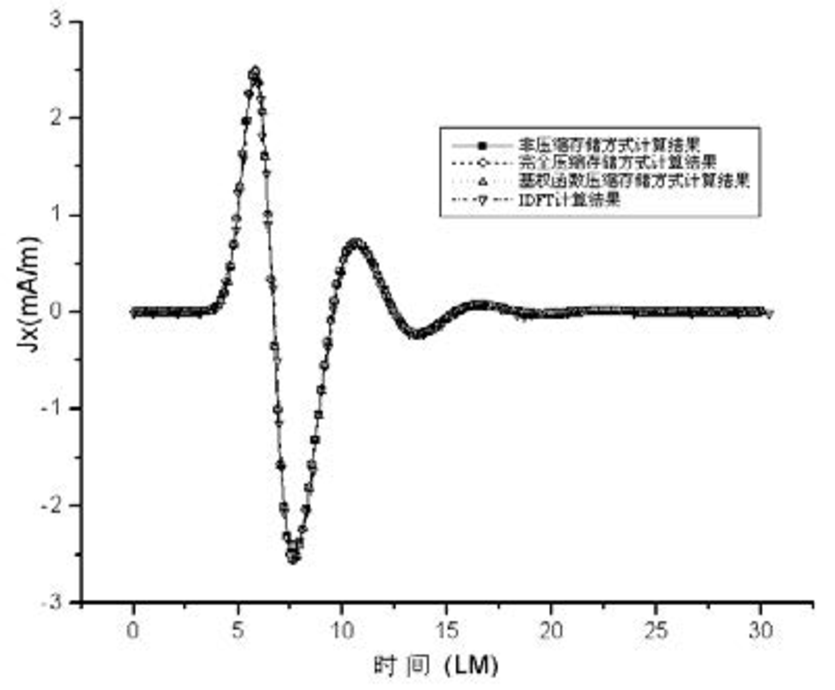
\includegraphics[width=6.77cm]{picd.pdf}
\subcaption{aa1}
\label{picd}
\end{subfigure}
\begin{subfigure}[b]{0.49\linewidth}
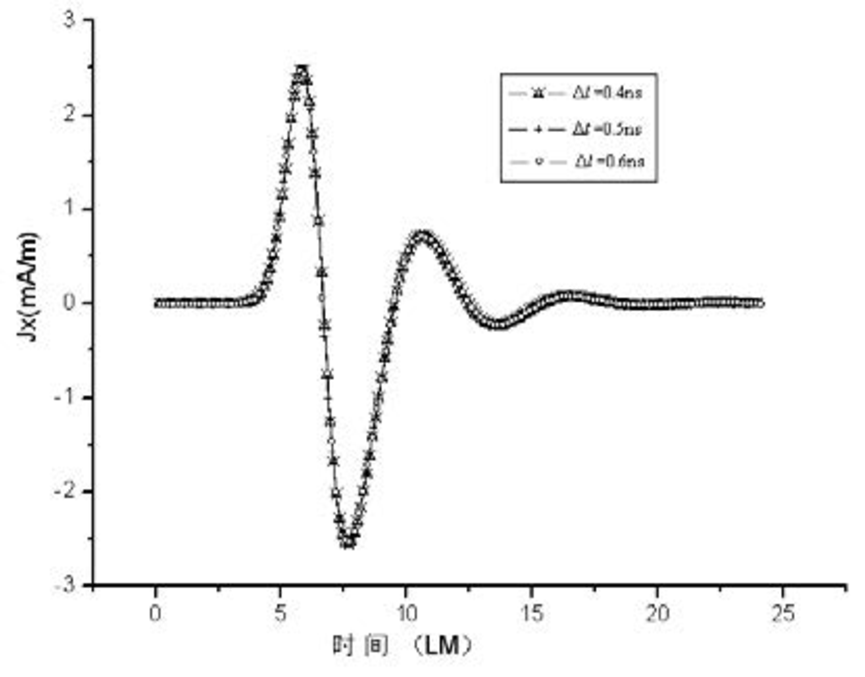
\includegraphics[width=7.04cm]{pice.pdf}
\subcaption{aa2}
\label{pice}
\end{subfigure}
\caption{曲线和曲线}
\label{fig2}
\end{figure}

\section{其它环境}
\begin{theorem}
定理1。
\end{theorem}
\begin{proof}
证明2
\end{proof}
\begin{corollary}
推论1
\end{corollary}
\begin{lemma}
引理2
\end{lemma}

\section{本章小结}

\blindtext